\chapter{Návrh ovládacích karet}
\section{Základní požadavky na Ovládací karty}
    Následující seznam popisuje základní požadavky na ovládací karty, seznam je seřazen podle priorit.
    \begin{enumerate}
        \item Schopno ovládat měřící karty.
        \item Možnost komunikace pomocí 100\,Mbit Ethernetu.
        \item Dostupnost komponentů.
        \item Cena komponentů.
    \end{enumerate}

    \section{Funkční bloky}
    \begin{figure}[ht!]
        \centering
        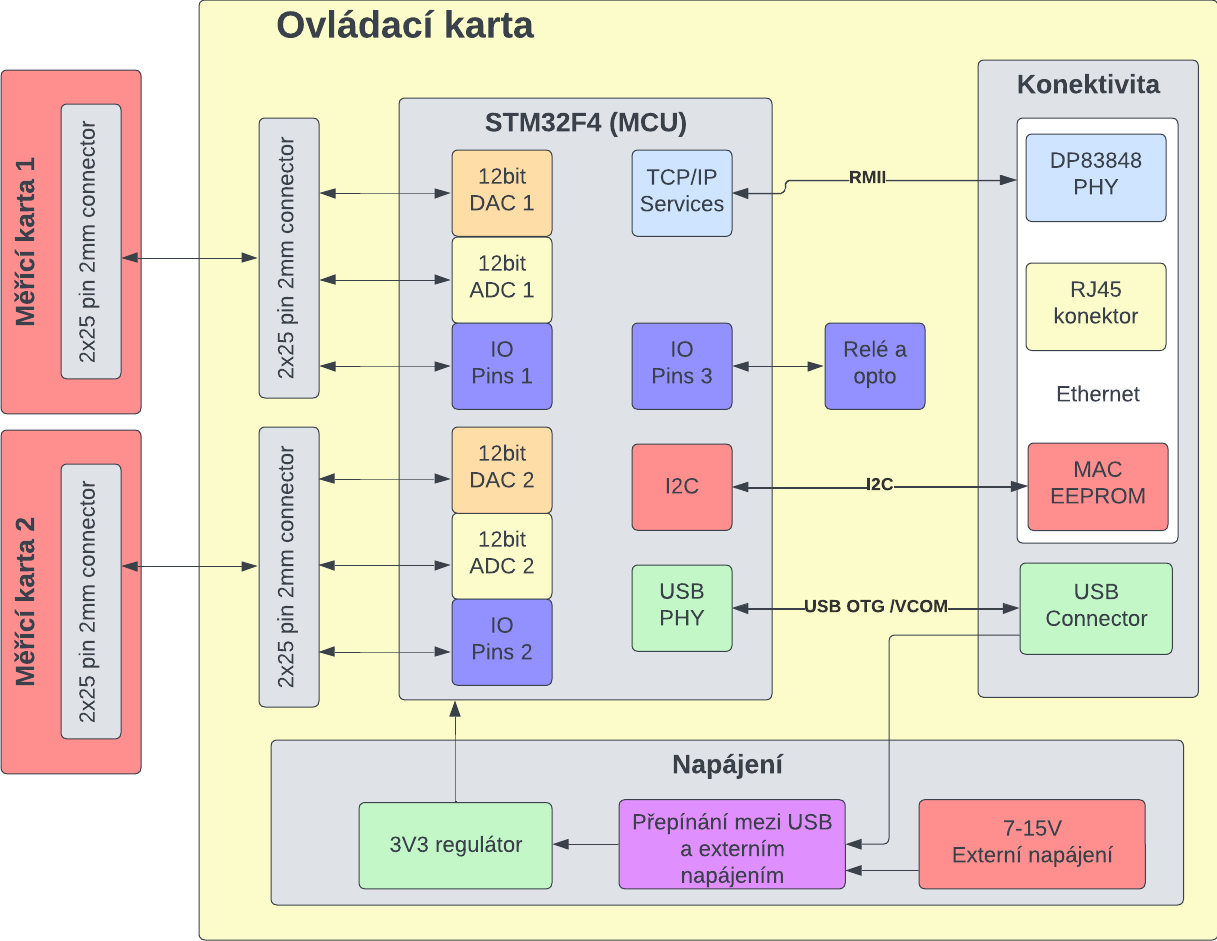
\includegraphics[width = 1\textwidth]{obrazky/ovladaci_karta_diag.png}
        \caption{Funkční diagram ovládací karty}
        \label{fig:Funkční diagram ovládací karty}
        
    \end{figure}

    Ovládací karta obsahuje několik pomyslných funkčních bloků (Obr. \ref{fig:Funkční diagram ovládací karty}).
    Jednotlivé bloky jsou podrobněji popsány v následujících kapitolách. Celé schéma k ovládací kartě je v příloze
    na konci tohoto dokumentu.

    \subsection{Mikrokontrolér a jeho periférie}
    Ovládací karta je založena na 32-bitovém mikrokontroléru STM32F407ZGT6 s Cortex M4 jádrem.
    Tento mikrokontrolér disponuje 114 I/O piny (3V3 logika), dvěma nezávislými 12-bit A/D a D/A převodníky,
    nativní podporou USB OTG a 100\,Mbit Ethernet MAC vrstvou. Právě díky těmto vlastnostem, je tento
    mikrokontrolér vhodný pro ovládání měřících karet a komunikaci s PC.\\

    Pro komunikaci s PC aplikací se primárně počítá s telnet serverem,
    který běží na mikrokontroléru. Nicméně pro debugovací
    účely je možno s ovládací kartou komunikovat i pomocí USB.
    K programování mikrokontroléru lze použít interface SWD nebo JTAG.\\

    Díky poměrně vysokému počtu I/O pinů,
    je možno pomocí jednoho mikrokontroléru ovládat napřímo až 2 měřící karty.
    Shift registry a multiplexery, umístěny na
    měřící kartě, jsou ovládány pomocí metody bit bangingu.
    Pro každou z měřících karet je použit dedikovaný D/A a A/D převodník\cite{MARTINT}.

    \subsubsection{D/A převodník}
    STM32F407ZGT6 nabízí dva 12-bit D/A převodníky s možností využití integrovaného bufferu v podobě
    invertujícího operačního zesilovače. Nicméně podle datasheetu
    je možné použít výstupní buffer pouze do velikosti kapacitní zátěže 50\,pF.
    Kapacitní zátěž D/A převodníku bude rovna parazitním kapacitám, které nelze jednoznačně určit
    a vstupní kapacitě 80 komparátorů (V+ proti GND). Každý z komparátorů má svou vstupní kapacitu
    přibližně 3\,pF. Dohromady tedy vznikne kapacitní zátěž minimálně 240\,pF.\cite{DAC}\\
    \begin{figure}[ht!]
        \centering
        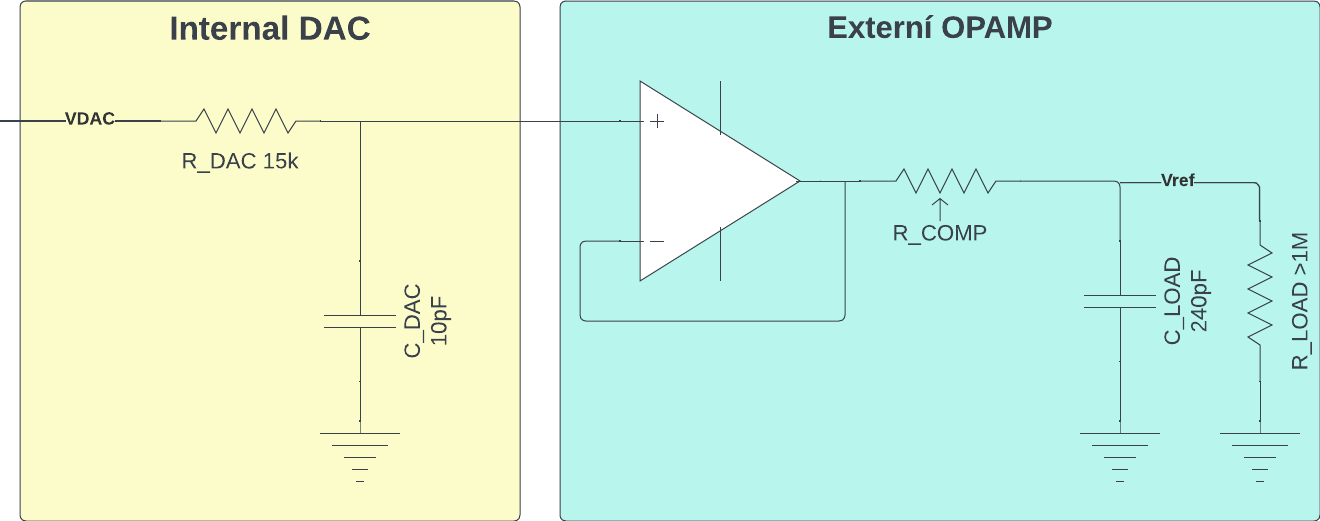
\includegraphics[width = 1\textwidth]{obrazky/DAC_OPAMP.png}
        \caption{DAC-externí zesilovač}
        \label{fig: DAC-externí zesilovač}
        
    \end{figure}

    Pro použití D/A převodníku je použit externí operační zesilovač v zapojení (Obr. \ref{fig: DAC-externí zesilovač}).
    V tomto zapojení je rychlost D/A převodníku limitována kapacitou pinu D/A převodníku C\_DAC (cca 10\,pF)
    a vnitřním odporem R\_DAC (cca 15\,k$\Omega$). Mezní kmitočet nezatíženého D/A převodníku pak lze určit následovně.
    \begin{equation}
        f_{max} = \frac{1}{2\pi \cdot  C_{dac} \cdot  R_{dac}} = \frac{1}{2\pi \cdot 10\,pF \cdot 15\,k\Omega} = 1,06\,MHz
    \end{equation}

    Protože kapacitní zátěž společně s výstupním odporem operačního zesilovače by mohla
    způsobit nestabilitu a s tím spojené nežádoucí oscilace v časové oblasti.
    Byl přidán do obvodu odpor R\_comp. Tento odpor přidá nulu do přenosové funkce a zabrání tak
    tomu, aby se fáze přenosové charakteristiky dostala do nuly (zajistí stabilitu).\\
    
    Protože datasheet neuvádí přesnou hodnotu výstupního odporu operačního zesilovače a nelze jednoznačně
    určit kapacitní zátěž, je odpor R\_comp realizován trimmerem. Trimmer je použit při kalibraci
    D/A převodníku. Kalibrace je prováděna tak, že se na výstupu D/A převodníku nastaví obdélníkový
    signál o frekvenci 500\,kHz a poté se trimmerem nastaví taková hodnota, aby v časové oblasti
    byl co nejmenší překmit\cite{DAC_stability,OPA_stability}.\\

    Nevýhodou kompenzačního rezistoru je však přidání nechtěného DC offsetu D/A převodníku. Tento offset by
    však měl být zanedbatelný, protože vstupní odpor komparátoru je vysoký. Zároveň je na výstup externího zesilovače
    připojen A/D převodník pro případnou kompenzaci offsetu.

    \subsubsection{Programování a debuging}
    Pro účely debugování a programování mikrokontroléru jsou zpřístupněny SWD a JTAG piny.
    Dále je možno modifikovat konfiguraci mikrokontroléru pomocí jumperů, které jsou propojeny
    s boot piny mikrokontroléru. Při normálním provozu se počítá s programováním pomocí SWD rozhraní.

    \subsubsection{Konfigurace hodinového signálu}
    
    Mikrokontrolér má vysokou variabilitu v konfiguraci hodinových signálů.
    K požadovaným funkcím ovládací karty je vhodné použít externí krystalový rezonátor, který bude
    připojen do High Speed Clock pinů mikrokontroléru. V případě ovládací karty bylo použit 8\,MHz
    krystalového rezonátoru ABM3B-8.000MHZ-D2-T společně s 2x27\,pF zatěžovacími kapacitory.\\

    \begin{figure}[ht!]
        \centering
        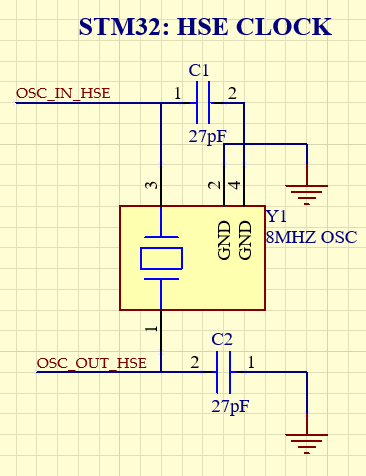
\includegraphics[height = 0.2\textheight]{obrazky/CLK_rezonator.png}
        \caption{8\,MHz krystalový rezonátor}
        \label{fig: MHz krystalový rezonátor}
    \end{figure}

    Pro jednodušší konfiguraci hodinových signálů mikrokontroléru bylo využito programu STM32CubeMX.
    Výsledná konfigurace hodinových signálů je znázorněna na následujícím obrázku.

    \begin{figure}[ht!]
        \centering
        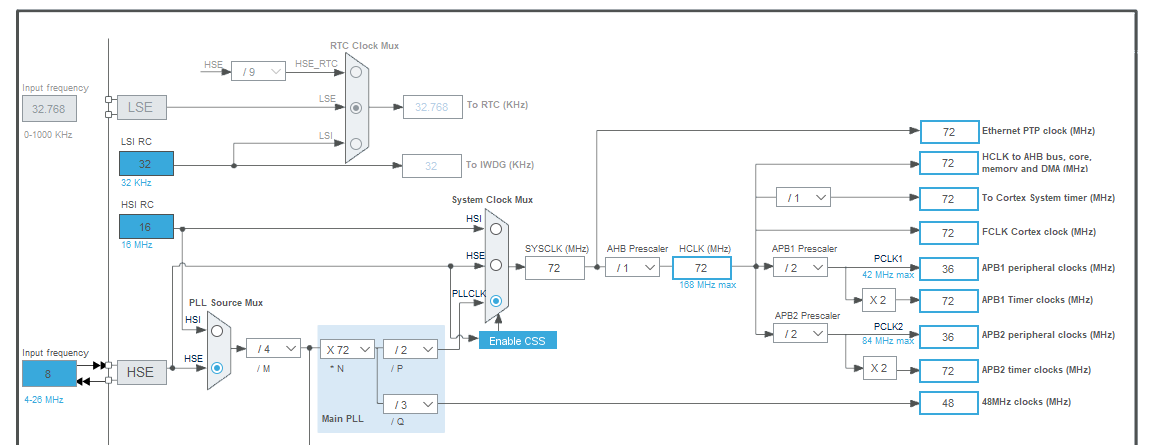
\includegraphics[width = 1\textwidth]{obrazky/CLK_config.png}
        \caption{Clock configuration}
        \label{fig: Clock configuration}
    \end{figure}

    \subsection{Konektivita}
    Ovládací karta je vybavena USB-micro a RJ45 konektorem. Umožňuje tak velmi snadné propojení s PC aplikací
    pomocí standardních USB a ethernetových rozhraní.

    \subsubsection{Ethernet}
    Pro zajištění ethernetového připojení je využito MAC
    vrstvy mikrokontroléru společně s fyzickou vrstvou (PHY)
    realizovanou pomocí čipu DP83848 a RJ45 konektoru s integrovaným transformátorem pro 100 BASE-T. Komunikace mezi
    mikrokontrolérem a DP83848 je realizováno pomocí RMII rozhraní. PHY vyžaduje pro svou správnou funkčnost
    100$\Omega$ diferenciální páry (viz. schéma ovládací karty v příloze).\\
    
    DP83848 vyžaduje pro svou činnost v RMII režimu připojení externího 50\,MHz oscilátoru.
    Výstup oscilátoru je zároveň přiveden na příslušný pin mikrokontroléru a slouží jako 
    hodinová reference.\\ 

    DP83848 je možno konfigurovat pomocí tzv. bootstrap pinů. DP83848 při svém startu zjišťuje
    logické úrovně bootstrap pinů a podle toho konfiguruje své parametry. Následující tabulka
    shrnuje nastavení bootstrap pinů použitých v ovládací kartě.

    \begin{table}[ht!]
        \resizebox{\columnwidth}{!}{%
        \begin{tabular}{|c|c|l|}
        \hline
        \textbf{PIN} & \textbf{Nastavení} & \textbf{Popis}                                   \\ \hline
        AN0 & 1 & AN0 a AN1 piny konfigurují, jakými možnostmi se bude zařízení prezentovat   při AutoNegotioation.   \\ \hline
        AN1 & 1 & Pro kombinaci AN0 = 1 a AN1 = 1 zařízení se prezentuje jako  10BASE-T a 100BASE-TX HALF/FULL duplex \\ \hline
        LED\_CFG     & 1                  & Konfiguruje chování LED na RJ45 konektoru.       \\ \hline
        MII\_MODE    & 1                  & DP83848 očekává RMII pro komunikaci s MAC vrstvou \\ \hline
        MDIX ENABLE  & 1                  & Interní pull up - MDIX (crossover) povolen       \\ \hline
        \end{tabular}%
        }
        \caption{Nastavení bootstrap pinů DP83848}
        \label{RMII settings}
        \end{table}


    Protože ani mikrokontrolér a ani DP83848 nenabízí jedinečnou MAC adresu je použita EEPROM,
    která má již od výrobce naprogramovanou jedinečnou MAC adresu.
    EEPROM používá ke komunikaci I2C protokol a při startu zařízení je MAC adresa
    načtena do MAC vrstvy mikrokontroléru. V mikrokontroléru je implementován telnet
    a http server a je využito LWIP stacku společně s HAL knihovnami a RTOS.\\

    \subsubsection{USB}
    Mikrokontrolér je vybaven fyzickou vrstvou pro USB OTG,
    je tak možné propojit datové signály přímo s USB-micro konektorem.
    Přestože je do USB konektoru vyveden ID pin, který slouží
    k rozlišení mezi host a device, využívá ovládací karta pouze device režim.
    Pro detekci připojení ovládací karty k USB portu je použit napěťový dělič, jehož výstup
    je přiveden do USB\_sense pinu mikrokontroléru. Napěťový dělič obsahuje rezistor o toleranci
    1\,\%. Tuto toleranci není nutno dodržet a tento rezistor byl použit pouze z důvodu nízké ceny
    a faktu, že se již v návrhu vyskytuje.\\

    Připojení pomocí USB slouží převážně k servisním účelům.
    Ovládací kartu lze napájet přímo z USB portu, přičemž napájení je opatřeno
    vstupním filtrem realizovaným feritovou perličkou a kondenzátorem (více v sekci o napájení).
    Obdobně jako u ethernetu je i zde nutno při návrhu PCB použít diferenciální páry
    pro datové signály (50\,$\Omega$). Každý ze signálů,
    který je vyveden na USB-micro konektor je opatřen TVS diodami pro ochranu
    proti ESD. \\

    \begin{figure}[ht!]
        \centering
        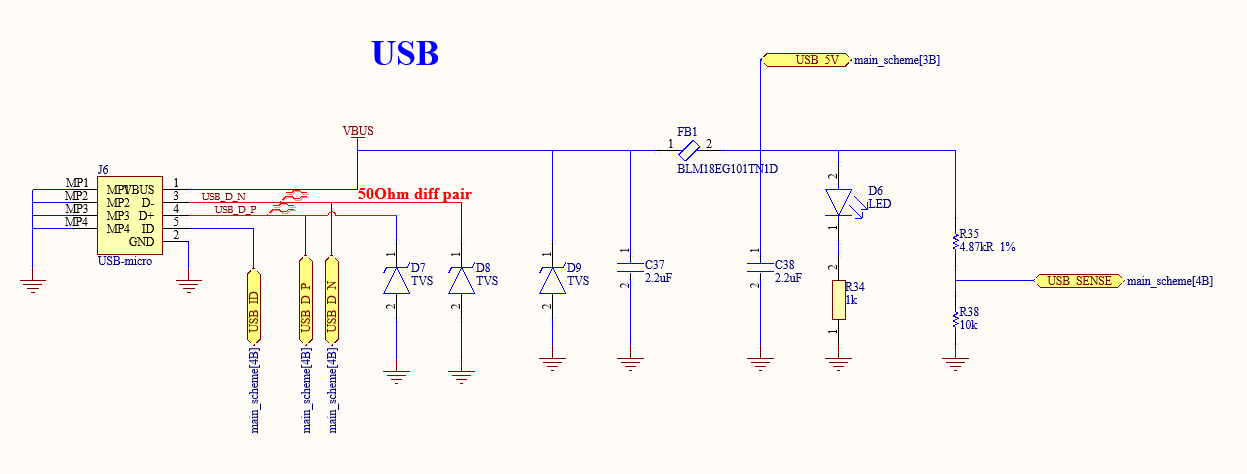
\includegraphics[width = 1\textwidth]{obrazky/USB.png}
        \caption{USB rozhraní}
        \label{fig: USB rozhraní}
    \end{figure}

\clearpage
    \subsection{Napájení}
    Při normálním provozu se počítá s externím napájení v rozmezí 7-15 VDC.
    Toto napětí je přivedeno na WAGO svorky. Napětí (ve schématu BOARD\_PWR)
    přivedeno na vstup nastavitelného regulátoru TLV76701DGNR. Funkce tohoto regulátoru je obdobná
    jako u regulátorů popsaných v sekci o měřící kartě. Výstup regulátoru je možné
    nastavit trimmerem v rozmezí přibližně od 2.8 do 3.45V (ve schématu 3v3\_MCUs).\\

    \begin{figure}[ht!]
        \centering
        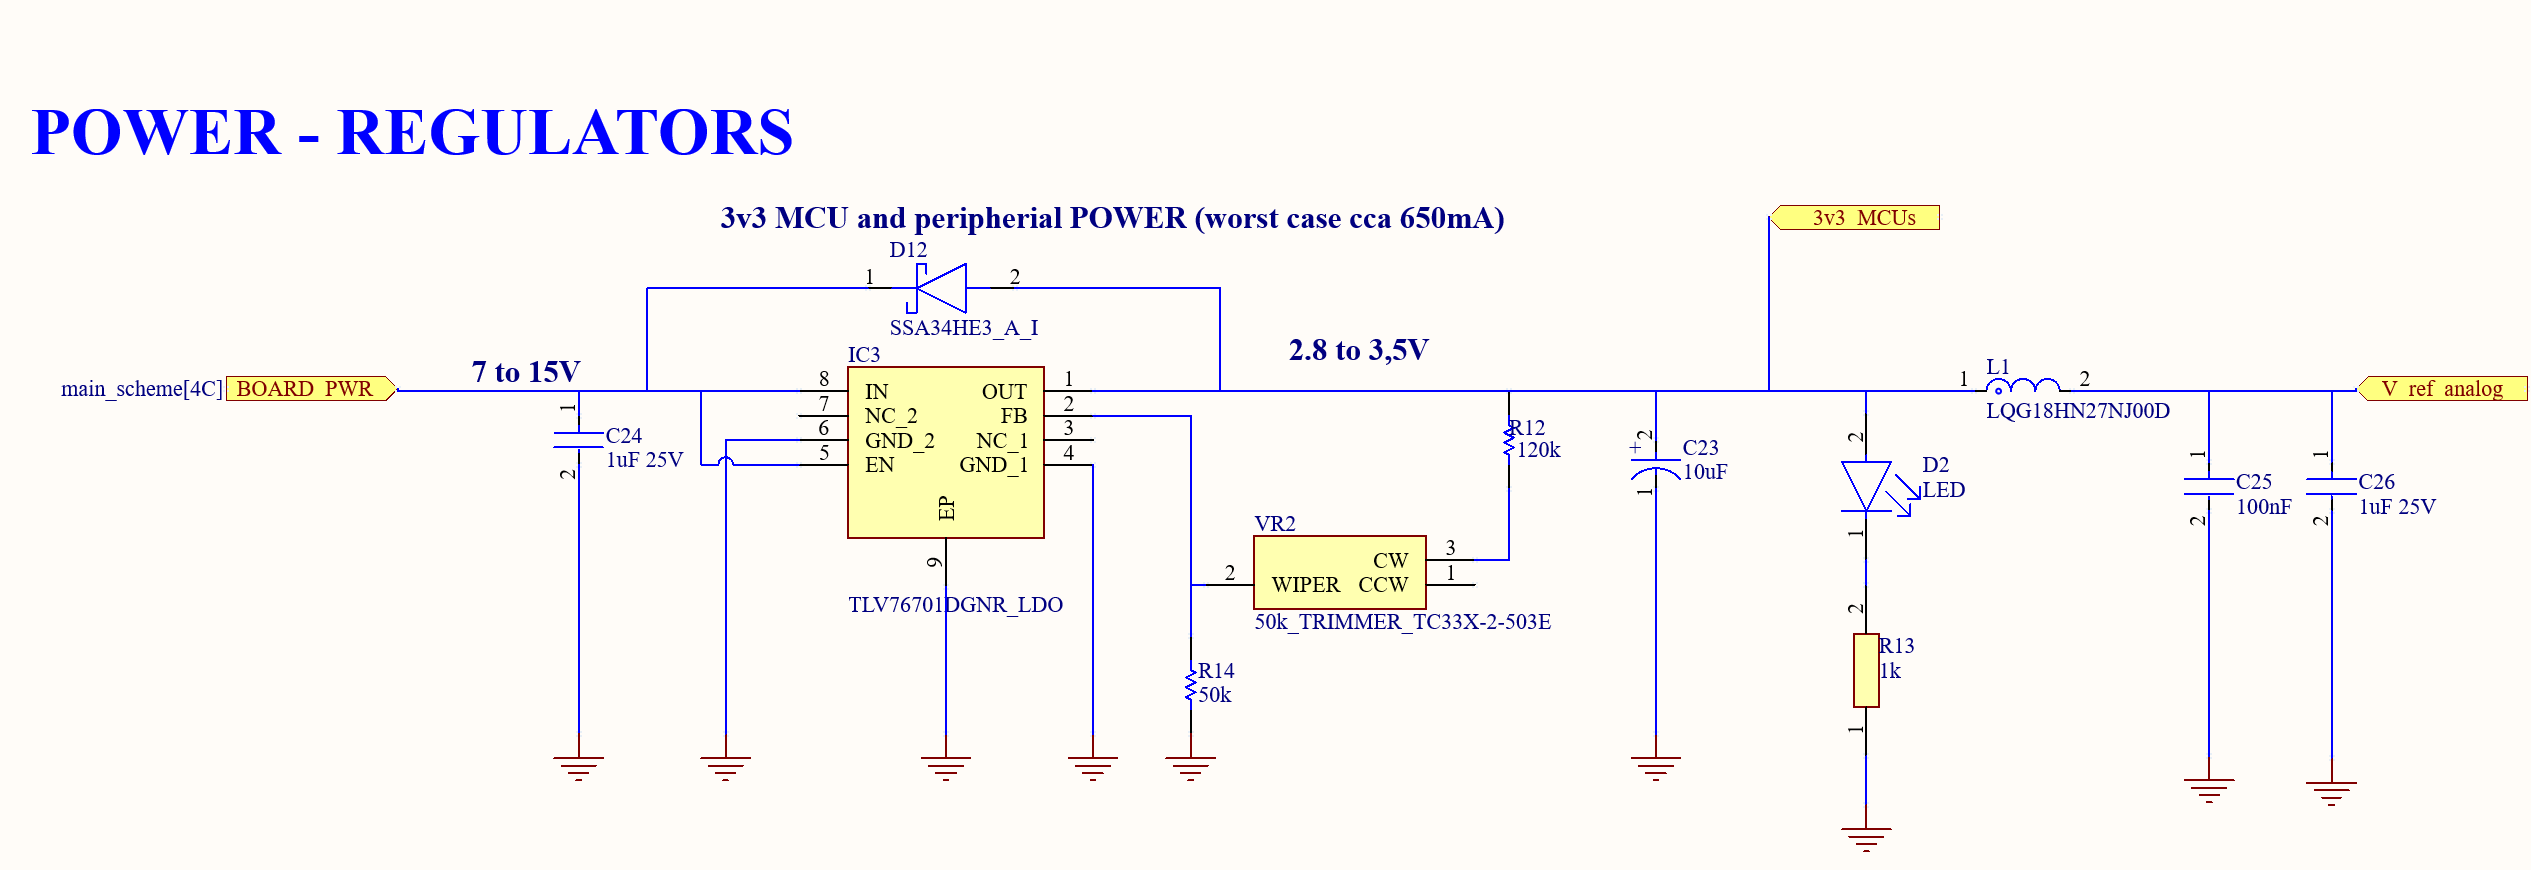
\includegraphics[width = 1\textwidth]{obrazky/PWR_REG_3V3.png}
        \caption{Regulátor napětí - 3V3 MCUs}
        \label{fig:Regulátor napětí - 3V3 MCUs}
    \end{figure}

    Takto regulované napětí je použito pro napájení všech doposud popsaných částí ovládací karty.
    Protože je vhodné aby referenční napětí (V\_ref\_analog),
    které mikrokontrolér používá  pro funkci A/D a D/A převodníků bylo co nejpřesnější, je
    napětí 3V3\_MCUs filtrováno dolní propustí realizovanou pomocí LC filtru.\\

    Očekávaný maximální proud fyzické vrstvy ethernetu je přibližně 150\,mA.
    Proudový odběr ovládací karty nelze jednoznačně určit,
    protože je závislý na firmwaru mikrokontroléru (deska není zatím fyzicky vyrobená a
    proudový odběr bude ověřen experimentálně).
    Nicméně se očekává, že by proud v nejhorším případě neměl přesáhnout 500\,mA. 
    Použitý regulátor by měl být schopen dodat do obvodu proud 1A, což by
    mělo být dostačující.\\ 
    
    Napětí je dále přivedeno na 2x25 pinový konektor,
    aby bylo možné napájet měřící a ovládací karty současně připojením napájecí napětí pouze
    na jednu z karet.\\

    Celý systém měřících a ovládacích karet může být napájen pomocí USB. V tomto případě je však přesnost
    měření limitována kvalitou USB napájení. Následující obrázek znázorňuje distribuci napájení
    ovládacích a měřících karet. Schéma však neodpovídá reálnému zapojení, protože jednotlivé
    komponenty jsou propojeny přes 2x25 pin konektory. Pro přehlednost jsou však konektory vynechány.
    \clearpage


    \begin{figure}[ht!]
        \centering
        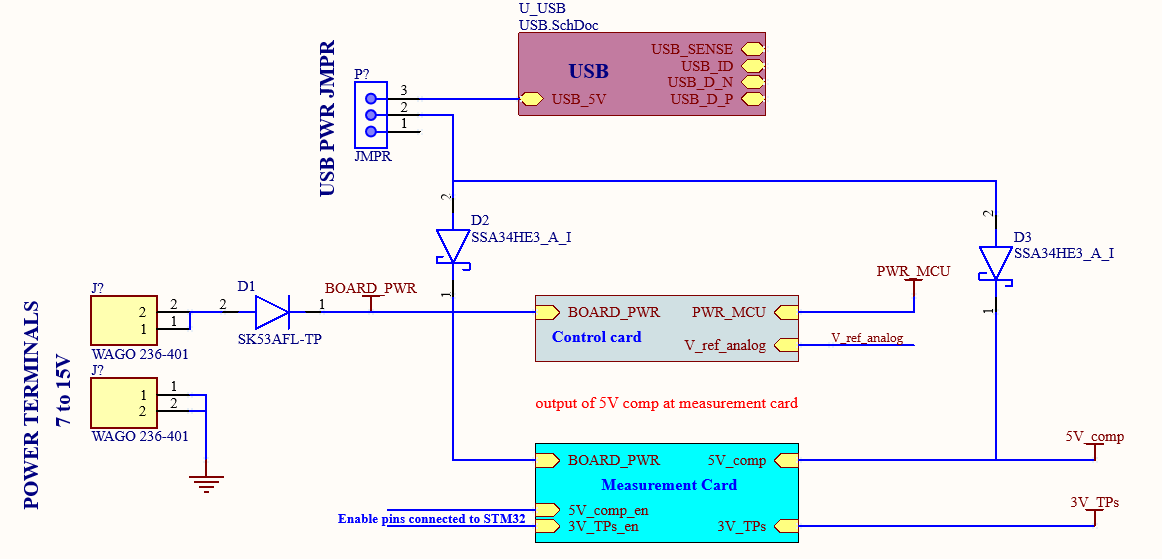
\includegraphics[width = 1\textwidth]{obrazky/USB_power_distr.png}
        \caption{Distribuce napájení}
        \label{fig:Distribuce napájení}
    \end{figure}

    V případě napájení pomocí USB je napětí BOARD\_PWR generováno z USB portu.
    Aby se zamezilo poškození všech připojených zařízení, které by mohlo potenciálně vzniknout připojením
    vyššího napětí na WAGO svorkách a USB současně, je do schématu připojena dioda D2. Dioda D1
    slouží jako ochrana k přepólování na vstupu WAGO svorek. Zároveň dioda D1 plní obdobnou funkci jako dioda D2
    nyní však pro ochranu zdroje napájení připojeného do WAGO svorek proti napětí na USB.
    V případě současného připojení externího napětí na WAGO svorky a USB portu, bude deska napájena
    vyšším z napětích.\\

    Napětí BOARD\_PWR je v případě napájení přes USB rovno přibližně:
    
    \begin{equation}
        V_{BOARD\_PWR} = V_{USB} - V_{D2} = 5V - 0.4V = 4.6V,
    \end{equation}
    Kde $V_{D2}$ je úbytek na diodě D2. Tento úbytek je pro diodu SSA34HE3\_A\_I roven přibližně 0.2V při proudu 1A
    a přibližně 0.4V při proudu 2A\\

    Úbytek napětí na regulátorech TLV76701DGNR je přibližně 0.8V.
    Součtem úbytků na diodě D2 a regulátoru lze 
    dosáhnou regulovaného výstupního napětí až 3.8V, což je dostatečné pro napájení všech regulátorů
    kromě regulátoru, který zajišťuje napětí 5V\_comp. Napětí 5V\_comp je tedy generováno přímo z USB portu přes 
    diodu D3. Dioda D3 má obdobný význam jako dioda D2, nyní však chrání USB port před vyšším napětím na výstupu
    regulátoru 5V\_comp v případě napájení z WAGO svorek. Z tohoto je patrné, že napětí 5V\_comp není nijak regulováno
    a je přímo závislé na napětí a rušení USB portu.
    V případě detekce napětí na USB\_sense pinu je komparátor 5V\_comp vypnut pomocí enable pinu.\\

    Pro možnost použití USB rozhraní pouze pro komunikaci (ne pro napájení),
    lze USB napájení rozpojit pomocí jumperu.\\

    





    %\subsection{Návrh PCB}
    %Tady bude sekce o návrhu PCB. Zatím není navrženo.
    %Ve výrobě jsou měřící karty, které by snad i s osazením měly být hotové do obhajoby semestrální práce.
    %Poté bude měřící karta otestována jejich funkčnost pomocí NUCLEO prototypových kitů.
    %Po verifikaci funkčnosti bude vyrobena ovládací karta.
    %Bude se pravděpodobně jednat o šestivrstvé PCB s řízenými impedancemi pro diferenciální páry.
    %    \subsubsection{USB routing}
    %Nějaký stručný popis vlivu impedance cesty na rychlost USB...
    %\subsubsection{Ethernet routing}
    %Nějaký stručný popis vlivu impedance cesty na rychlost Ethernetu. Signal integrity atd..
    %\subsubsection{STM32F4 routing}
    %Vliv decoupling kondenzátorů.
    %\subsubsection{Fyzické rozměry}
    %Na rozdíl od měřících karet, kde byl kladen důraz na maximální výšku karty z důvodu roztečí bRC pinů, nejsou
    %kladeny na ovládací karty žádné omezení, protože ovládací karty budou propojeny s měřícími kartami
    %pomocí páskových vodičů. Rozměry by však měly být co nejkompaktnější. Propojit měřící karty s bRC piny pomocí
    %páskových vodičů nebylo žádoucí z důvodu vnášení chyby měření do systému.
    %\clearpage


\chapter{Algoritmizace a měřící procedury}
Jak již bylo zmíněno v kapitole o systémové koncepci a na obr.\ref{fig:Systémová koncepce}.
Jednotlivé ovládací karty jsou propojeny pomocí ethernetového rozhraní do switche.
Pro správnou funkčnost testeru je zde použit spravovatelný switch, který mimo jiné umožňuje
získat informace o své MAC tabulce. MAC tabulku společně s protokolem ARP lze využít pro
přiřazení čísla portu ethernetového switche k IP adrese připojených ovládacích karet. Tímto způsobem
lze přiřadit jednotlivé ovládací karty k jednotlivým řadám bRC pinů bez nutnosti dodatečné konfigurace
či různému kódování řad.\\

Z pohledu celého systému je hlavním řídícím prvkem PC aplikace.
Ovládací karty společně s měřícími kartami nabízejí PC aplikaci high level služby.
Tyto high level jsou dostupné díky telnet server ovládací karty. Pojmem high level služby
si lze představit například telnet příkaz \#SET;IMPEDANCE;HIGHZ;PINS;ALL ,tento příkaz odešle
PC aplikace některé z ovládacích karet. Karta nastaví všechny bRC piny na připojených měřících kartách
do vysoké impedance a odešle potvrzení zpět řídící aplikaci pomocí telnet příkazu následovně
\#SET;IMPEDANCE;HIGHZ;PINS;ALL;ACK. Na následujícím obrázku lze pozorovat složitější příklad mezi
PC aplikací a ovládacími kartami.

\begin{figure}[ht!]
    \centering
    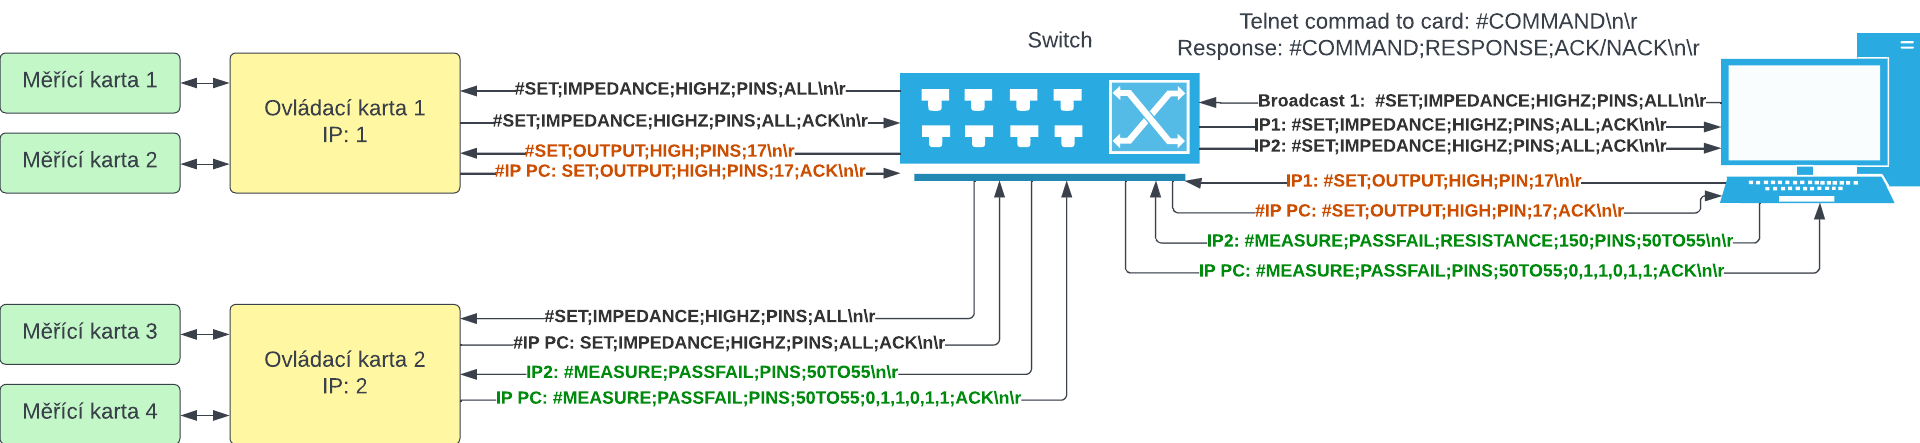
\includegraphics[width = 1\textwidth]{obrazky/telnet_communication.png}
    \caption{Telnet komunikace}
    \label{fig:Telnet komunikace}
\end{figure}

V příkladu na obr. \ref{fig:Telnet komunikace} PC aplikace nejprve zašle všem připojeným ovládacím kartám
(broadcast) příkaz pro nastavení všech pinů do vysoké impedance. Poté PC aplikace čeká až obdrží potvrzení 
od všech připojených karet. Následně nastaví pomocí ovládací karty č. 1 pin č. 17 na měřící kartě jako výstup.
Po obdrženém potvrzení ok ovládací karty 1 odešle PC aplikace dotaz ovládací kartě 2. Tento dotaz
(\#MEASURE;FASTVALUE;RESISTANCE;150;PINS;50TO55) by se do lidské řeči dal přeložit následovně. Nastav 
výstup D/A převodník tak, aby hodnota napětí změřená na komparátoru odpovídá odporu 150 ohmů.
Následně vrať výstupní data multiplexeru pro piny 50 až 55.
Z odpovědi ovládací karty lze určit zda mezi pinem (řada 1 pin 17)
a piny (řada 3 piny 50-55) je odpor odpor propojení menší než 150 ohmů.\\ 

Z příkladu je také patrné, že karty samotné neinicializují komunikaci a komunikují pouze s PC aplikací.
Tímto je sice poněkud redukován výpočetní výkon systému, ale zároveň se řízení velmi zjednodušuje.
Řízení pomocí PC aplikace také zajišťuje synchronizaci mezi jednotlivými kartami.

\section{Mód PASS/FAIL}
V sekci (Volba velikosti odporu děliče Rout) byly zmíněny dva módy, ve kterých tester funguje.
Prvním z módu je PASS/FAIL mód. V tomto módu používá obsluha externí sondu připojenou k pinu č. 80
měřící karty připojené k ovládací kartě č.1. Obsluha je vyzvána k připojení externí sondy k 
určité testovací jehle (probe). Tester následně otestuje, které propojení mezi bRC piny a sondou splňuje požadavky
na mezní hodnotu odporu cesty.\\

Naměřená jsou odesílána do PC aplikace, která výsledky porovnává
s konfiguračními soubory a v závislosti na výsledku informuje obsluhu o dalším postupu.
Informování obsluhy je realizováno akusticky (obdobně jako continuity test u multimetru)
a vizuálně na displeji. Celý systém tak musí provést měření, co nejrychleji, aby aplikace byla schopna informovat
obsluhu v reálném čase s co nejnižší odezvou.\\

Pro tento mód testeru je možné použít obdobný postup jako na obr. \ref{fig:Telnet komunikace}.
Zde se místo pinu 17 použije pin 80 a místo pinů 50-55 se postupně proměří všechny cesty po skupinách
40 pinů (zdůvodnění proč zrovna 40 pinů je v sekci o návrhu měřící karty).\\

PC aplikace postupně ukládá naměřená data z jednotlivých měřících karet do matice o rozměru 50x78 (rozměr používaných bRC pinů).
A následně je porovnává s maticí vytvořenou z konfiguračních souborů. Na obrázku níže jsou zobrazeny matice naměřených
a očekávaných hodnot. Matice má pro názornost rozměr pouze 3x3.

\begin{figure}[ht!]
    \centering
    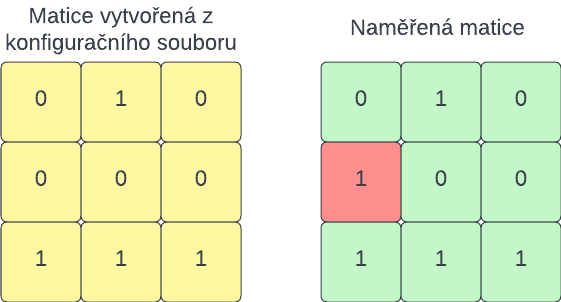
\includegraphics[width = 0.7\textwidth]{obrazky/MATRIX_COMPARISSON.png}
    \caption{PASS/FAIL matrix}
    \label{fig:PASS/FAIL matrix}
\end{figure}

V matici naměřených hodnot jsou zeleně znázorněny výsledky, které se shodují s předpokládanými hodnotami.
Červeně jsou naopak zobrazeny hodnoty, které jsou rozdílné. Hodnota 0 znamená, že mezi externí sondou (probe pinem)
a bRC pinem odpovídající pozici v matici není propojení cesty nižší jak zvolená mezní hodnota odporu.
Naopak hodnota 1 znamená, že mezi sondou a bRC pinem je propojení cesty v požadovaném rozsahu. Z výsledků
měření na obr. \ref{fig:PASS/FAIL matrix} je tedy patrné, že zkoumaný probe pin je někde špatně připojený do 
bRC pinu (řada 2, sloupec 1). Z konfiguračních souborů lze zjistit i název signálu, který vede do tohoto probe
popřípadě bRC pinu a obsluhu informovat o tom, mezi kterými signály a piny vznikl problém.
Tímto postupem se proměří všechny probe piny (každý probe pin má sadu těchto matic).\\


\section{Mód měření přesné hodnoty odporu}
Tento mód se oproti PASS/FAIL módu liší tím, že zde nejsou kladeny žádné nároky na čas měření, protože proces
je plně automatizován a měření probíhá pouze mezi bRC piny.
V tomto módu však tester zjišťuje co nejpřesnější hodnotu propojení cest.
Obdobně jako v PASS/FAIL módu je výsledkem matice propojení, kde jsou nyní však místo jedniček a nul hodnoty
změřeného odporu. Matice vytvořená z konfiguračních dat však zůstává stejná, protože data v sobě nemají
žádné hodnoty odporu propojení. Lze pak stanovit určitý treshold obdobně jako při PASS/FAIL režimu a
určit tak, zda naměřené hodnoty odpovídají očekávaným datům. Následující obrázek ukazuje 
vzniklé matice pro jeden bRC pin pro zvolený treshold 30\,$\Omega$.\\

\begin{figure}[ht!]
    \centering
    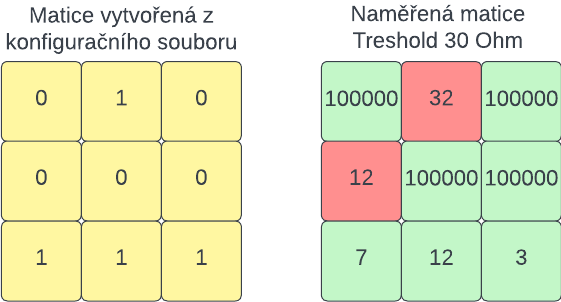
\includegraphics[width = 0.7\textwidth]{obrazky/MATRIX_TRUEVALUE.png}
    \caption{TRUEVALUE matrix}
    \label{fig:TRUEVALUE matrix}
\end{figure}

V obr. \ref{fig:TRUEVALUE matrix} lze najít hodnoty odporu 100000$\Omega$. Tyto hodnoty však neodpovídjí reálné hodnotě propojení
cest, ale je značí že měřená hodnota odporu je mimo rozsah testeru a lze tak předpokládat, že zde žádné propojení není.
Dále je zde možno najít červené pole s hodnotou 32$\Omega$. Podle matice vytvořené z konfiguračního 
souboru by tato cesta měla být propojená. Nicméně pro zvolený treshold 30$\Omega$ je tato hodnota odporu propojení
považována za příliš vysokou a vyhodnocena jako chybné propojení.\\

Přesná hodnota odporu se zde měří tak, že pro každou skupinku pinů, je vytvořena rampa D/A převodníku a 
monitoruje se, při jaké hodnotě napětí na D/A převodníku se překlopí výstup komparátoru daného pinu. Aby se 
minimalizovala chyba vzniklá úbytkem napětí na P-channel mosfetu (viz kapitola o návrhu měřící karty),
lze zároveň využít rampu D/A převodníku pro změření přesného výstupu napětí bRC pinu a výsledek měření tak vztáhnout
přímo k napětí na bRC pinu.\\

\chapter{Řídící PC aplikace}
Pro účely testeru byla vyvinuta PC aplikace založená na programovacím jazyku python. Tato aplikace umožňuje
nejen komunikovat s testerem a provádět měření, ale také převádět vstupní CAD, CAM, gerber a různé textové konfigurační
soubory do vhodného formátu pro účely testeru.\\

Aplikace se skládá ze 3 hlavních záložek (Routing, Probe Test a Auto Test) v horním levém rohu. V semestrální práci Je
dokončena funkce pouze záložky routing.

\section{Záložka routing}
Tato část řídící aplikace má na starosti převod všech vstupních dat do vhodného grafického zobrazení a vytvoření
propojovacích matic (viz obr. \ref{fig:TRUEVALUE matrix} a Obr.\ref{fig:PASS/FAIL matrix}).
Ve svém GUI je záložka koncipována tak, aby obsluha testu byla schopna identifikovat různá propojení bRC a probe pinů.
Zároveň by mělo být možné na základě tohoto GUI zapojit celou fixture část.\\

\begin{figure}[ht!]
    \centering
    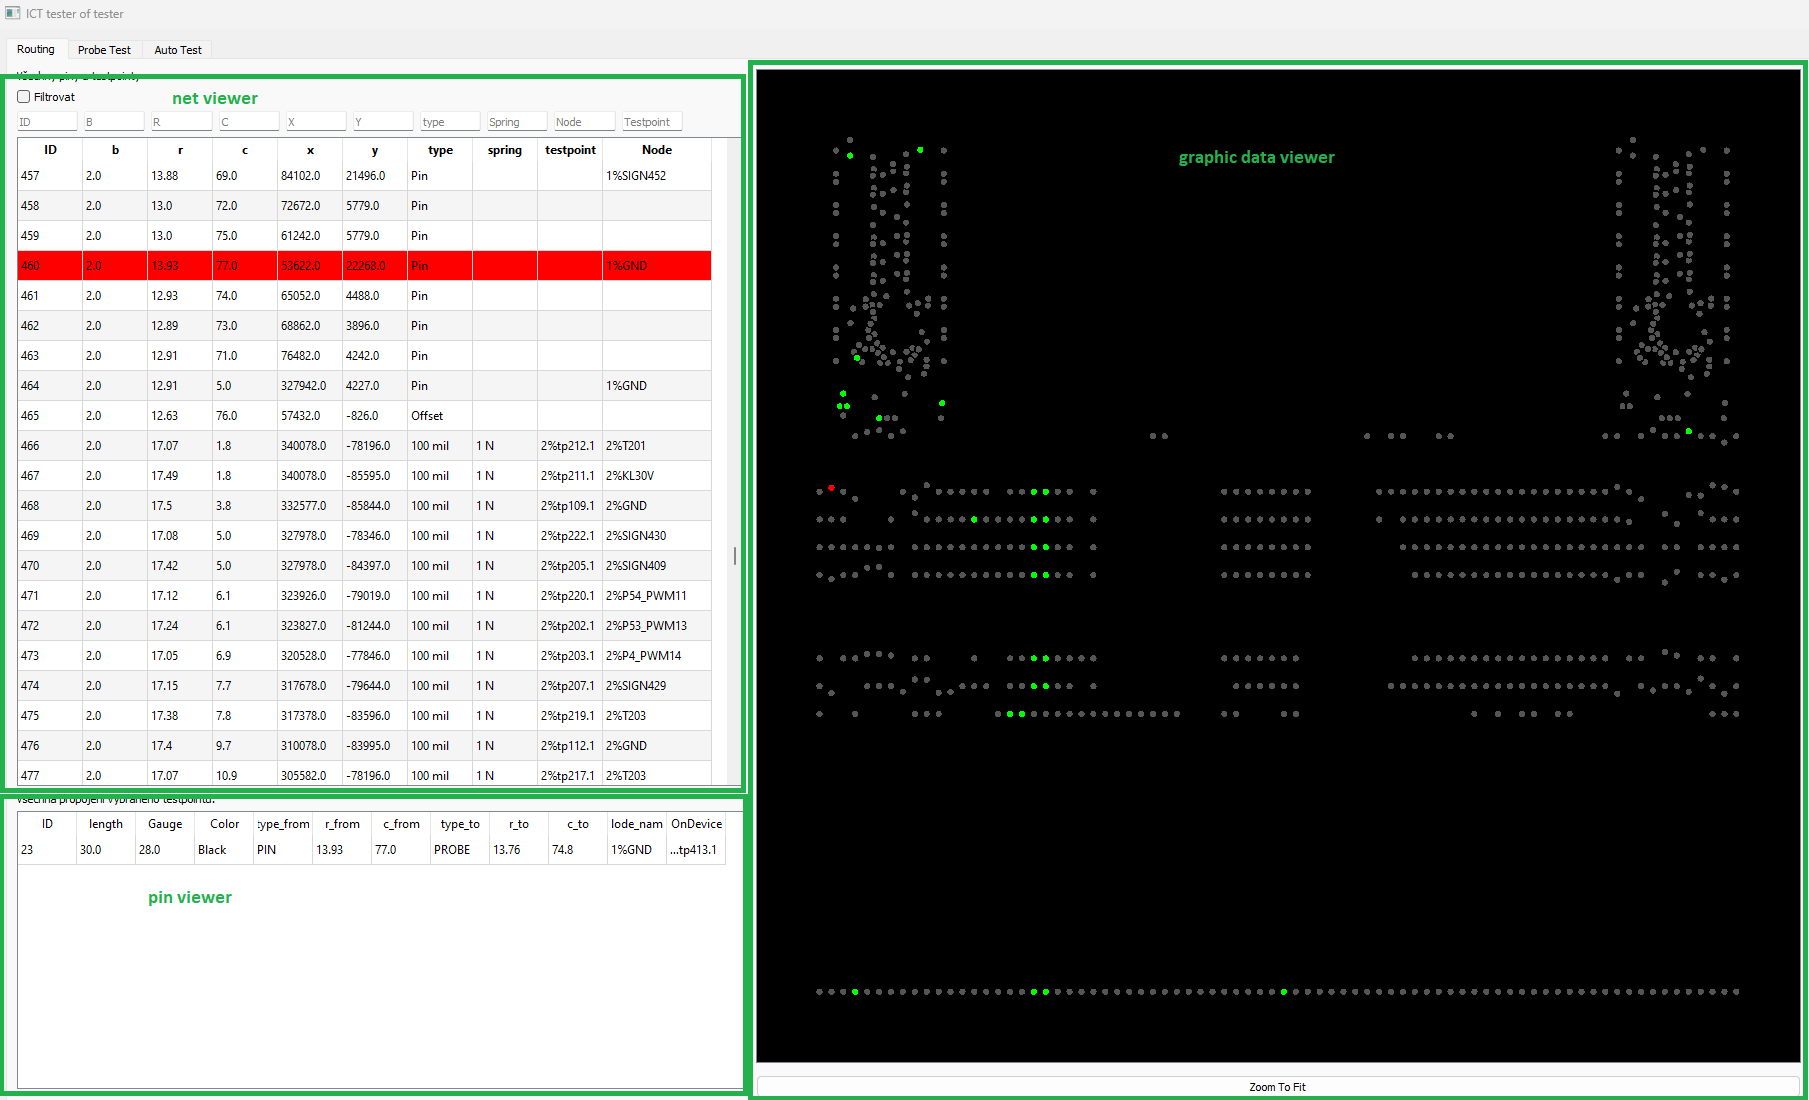
\includegraphics[width = 1\textwidth]{obrazky/PC_AP_top_view.png}
    \caption{PC aplikace - záložka routing}
    \label{PC aplikace - záložka routing}
\end{figure}

Záložka se skládá ze 3 hlavních částí (net viewer, pin viewer a data graphics viewer).
V části netviewer jsou zobrazeny všechny bRC a probe piny (jsou zde i jiné piny, které nejsou diskutovány v diplomové práci).
Každý pin zde má svou polohu vyjádřenou dvěma způsoby. Prvním způsobem je značení pomocí bRC. Toto označení je
vztaženo k mřížce, kterou tvoří spodní část fixture (obr. \ref{fig:ICT_tester}). Protože jednotlivé piny mají svou toleranci
a nemusí ležet přímo v bodě mřížky, je označení bRC nepřesné a je zaokrouhleno k nejbližšímu bodu mřížky.
Druhým a přesným způsobem je označení pomocí x a y souřadnic.\\

Některé piny mají neprázdná pole označení ve sloupci testpoint.
Toto označení znamená, že se jedná o probe pin a bude ho nutné otestovat externí sondou. Zároveň probe piny
mají ve sloupci type průměr testovací jehly (bRC piny mají označení pin). Dále je zde vidět Node (uzel) do kterého pin patří.\\

Po kliknutí do příslušného řádku v části netviewer se v části graphic data viewer zobrazí červeně zvolený pin
a zároveň zeleně všechny probe a bRC piny se stejným označením node (obr. \ref{PC aplikace - záložka routing}).
V části graphic data viewer zároveň lze klikat myší na jednotlivé piny a tím je označit v sekci netviewer.
Takto lze jednoduše procházet zapojení fixture části. Část graphic data viewer umožňuje různě přibližovat a posouvat
zobrazení.\\

V části pin viewer jsou zobrazeny podrobné informace o vybraném (červeném) pinu.
Každý řádek v této sekci (může jich být libovolný počet) obsahuje informace o propojení zvoleného červeného pinu s nějakým
dalším pinem. Na obr(\ref{PC aplikace - záložka routing}) je patrné, že v části pin viewer je pouze jeden řádek, ale zároveň
z části graphic data viewer je jasně vidět, že uzel 1\%GND obsahuje daleko více pinů. To je způsobeno tím,
že uzly nejsou vždy tvořeny paralelním propojením všech pinů. Dále aby bylo možno fixture zapojit, obsluha musí v části
pin viewer vidět pouze propojení kam dále má vést propojení. Zobrazeny jsou tedy pouze cesty, které vedou z tohoto pinu.
Toto je patrné i z informací v příslušném řádku části pin viewer. V obr.(\ref{PC aplikace - záložka routing}) jsou ve sloupcích
r\_from a c\_from (značí z kterého pinu vede cesta) stejná data jako ve sloupcích r a c v části netviewer. Jedná se tudíž
o červený vybraný pin. Sloupce r\_to a c\_to jsou souřadnice pinu, kam má vést další cesta. Po kliknutí do řádku
v části pin viewer se v části graphic viewer znázorní pomyslné propojení (\ref{PC aplikace - Zobrazení cesty}).
Zároveň lze z řádku v sekci pin viewer vyčíst data o délce, typu a barvě použitého propojovacího drátu.
\begin{figure}[ht!]
    \centering
    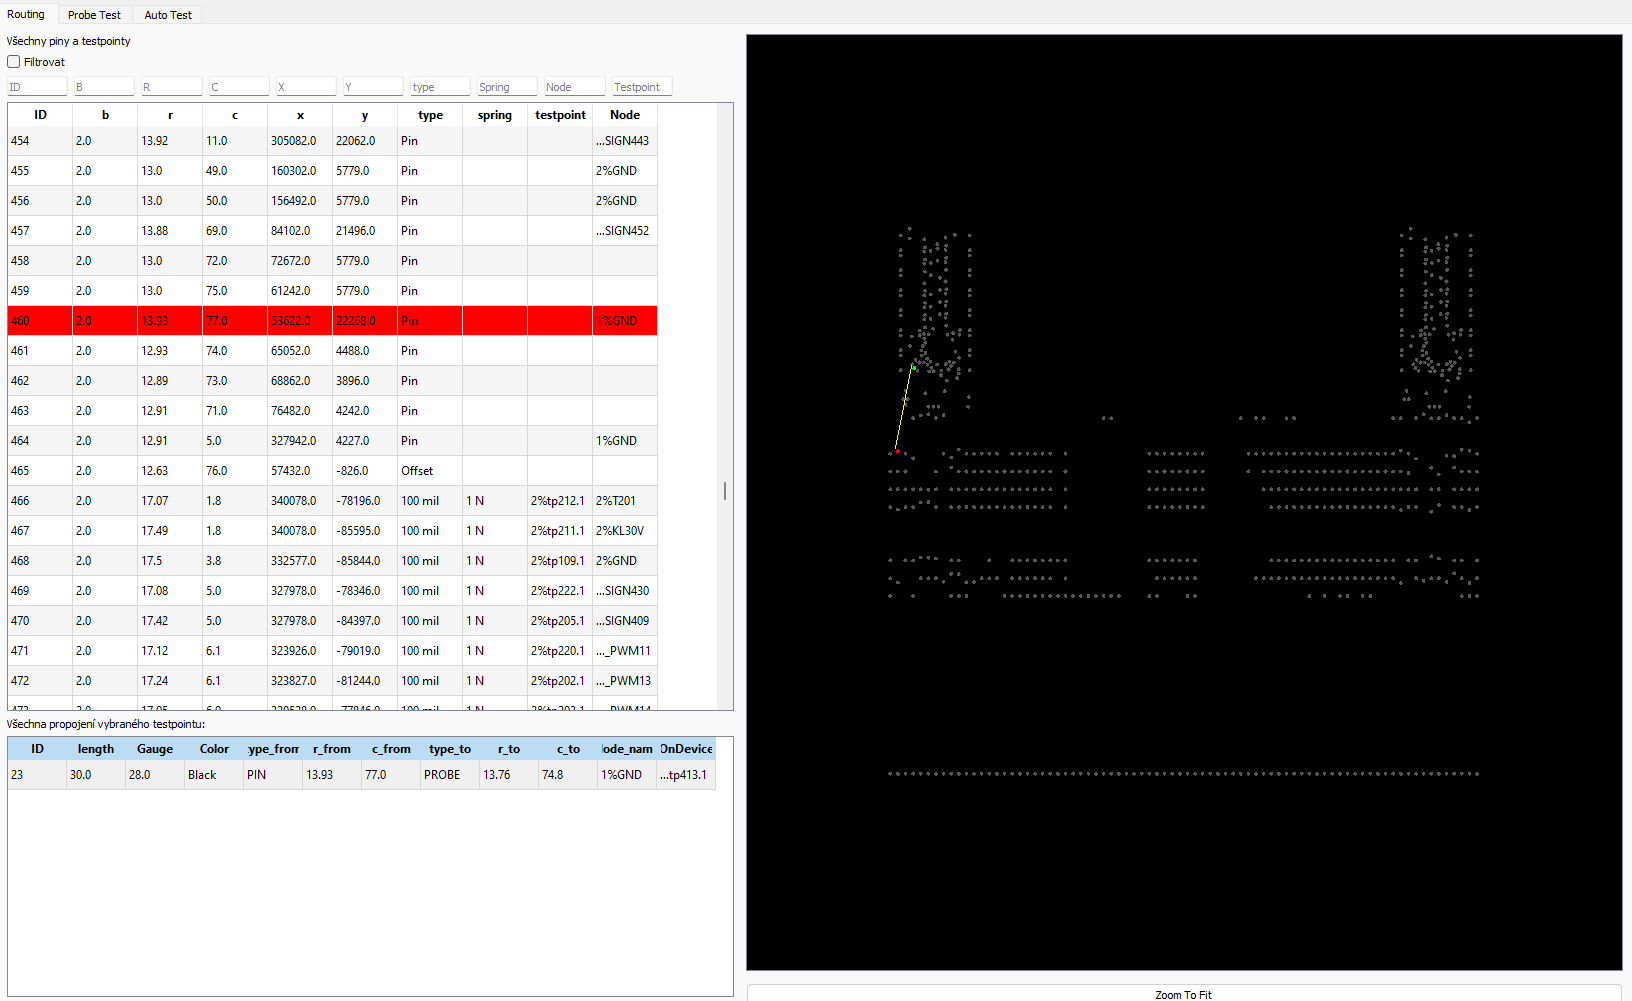
\includegraphics[width = 0.9\textwidth]{obrazky/PC_AP_top_only1.png}
    \caption{PC aplikace - Zobrazení cesty}
    \label{PC aplikace - Zobrazení cesty}
\end{figure}